\documentclass[12pt]{book}
\usepackage{amssymb}
\usepackage{amsmath}
\usepackage{amsthm}
\usepackage{amsfonts}
\usepackage{mdframed}
\usepackage{tikz-cd}
\usepackage{stmaryrd}
\usepackage{hyperref}
\setlength{\evensidemargin}{0.25in}
\setlength{\oddsidemargin}{0.25in}
\setlength{\textwidth}{6in}
\parskip0.2em

\newmdtheoremenv{theorem}{Theorem}[section]
\newmdtheoremenv{lemma}[theorem]{Lemma}
\newmdtheoremenv{proposition}[theorem]{Proposition}
\newmdtheoremenv{corollary}[theorem]{Corollary}
\newmdtheoremenv{conjecture}[theorem]{Conjecture}
\theoremstyle{remark}
\newtheorem{assumption}[theorem]{Assumption}
\newtheorem{property}[theorem]{Property}
\newmdtheoremenv{remark}[theorem]{Remark}
\theoremstyle{definition}
\newmdtheoremenv{definition}[theorem]{Definition}
\newtheorem{example}[theorem]{Example}
\newtheorem{exercise}{Exercise}[section]
\numberwithin{equation}{section}
\allowdisplaybreaks[1]

%Peng's command
\newcommand{\MW}{Milnor-Witt\ }
\newcommand{\rMW}{\mathrm{MW}}
\newcommand{\KMW}{\mathrm{K}^\mathrm{MW}}
\newcommand{\KM}{\mathrm{K}^\mathrm{M}}
\newcommand{\sKMW}{\mathscr{K}^\mathrm{MW}}
\newcommand{\tbb}[1]{\widetilde{\mathbb{#1}}}
\newcommand{\wt}[1]{\widetilde{#1}}
\newcommand{\Spec}{\mathrm{Spec}\ }
\newcommand{\af}{\mathbb{A}}
\newcommand{\afnz}[1]{\mathbb{A}^{#1}\setminus \{0\}}
\newcommand{\nonZero}{\setminus \{0\}}
\newcommand{\cO}{\mathcal{O}}
\newcommand{\cC}{\mathcal{C}}
\newcommand{\cD}{\mathcal{D}}
\newcommand{\cX}{\mathcal{X}}
\newcommand{\cY}{\mathcal{Y}}
\newcommand{\bR}{\mathbb{R}}
\newcommand{\bC}{\mathbb{C}}
\newcommand{\bZ}{\mathbb{Z}}
\newcommand{\bfZ}{\mathbf{Z}}
\newcommand{\tbZ}{\tbb{Z}}
\newcommand{\inv}{^{-1}}%
\newcommand{\Gm}{\mathbb{G}_m}
\newcommand{\tGm}{\tbb{G}_m}
\newcommand{\Sp}{\mathrm{Sp}}
\newcommand{\GL}{\mathrm{GL}}
\newcommand{\SL}{\mathrm{SL}}
\newcommand{\MSp}{\mathrm{MSp}}
\newcommand{\BSp}{\mathrm{BSp}}
\newcommand{\SH}{\mathcal{SH}}
\newcommand{\Da}{D_{\af^1}}
\newcommand{\Daba}[1]{D(Ab_{\af^1}(#1))}
\newcommand{\DM}{\mathrm{DM}}
\newcommand{\DMt}{\widetilde{\mathrm{DM}}}
\newcommand{\M}{\mathrm{M}}
\newcommand{\Mt}{\wt{\mathrm{M}}}
\newcommand{\Meta}{\wt{\mathrm{M}}_{\eta}}
\newcommand{\HH}{\mathrm{H}_{\rMW}}
\newcommand{\Heta}{\mathrm{H}_{\eta}}
\newcommand{\sBra}[1]{\left[#1\right]}
\newcommand{\aBra}[1]{\left<#1\right>}
\newcommand{\llBra}[1]{\llbracket #1 \rrbracket
}
\newcommand{\Set}{\mathbf{Set}}
\newcommand{\Top}{\mathbf{Top}}
\newcommand{\Hom}{\mathrm{Hom}}
\newcommand{\Ker}{\mathrm{Ker}}
\newcommand{\Fun}{\mathrm{Fun}}
\newcommand{\Spc}{\mathcal{S}pc}
\newcommand{\gy}{\rm{Gysin}}
\newcommand{\xr}[1]{\xrightarrow{#1}}

\newcommand{\AZ}{\mathbb{A}\mathcal{Z}}
\newcommand{\bfZa}{\mathbf{Z}_{\mathbb{A}^1}}

\raggedbottom

\title{Seeing the Mountain}
\author{Keyao Peng}



\begin{document}
\begin{titlepage}
\begin{center}
{\huge\bfseries Seeing the Mountain \\}
% {\Large A Journey Through Post-Modern Geometry \\}
 % ----------------------------------------------------------------
 \vspace{1.5cm}
 {\Large\bfseries Keyao Peng}\\[5pt]
 keyao.peng@ube.fr\\[14pt]
  % ----------------------------------------------------------------
 \vspace{2cm}
 % ----------------------------------------------------------------
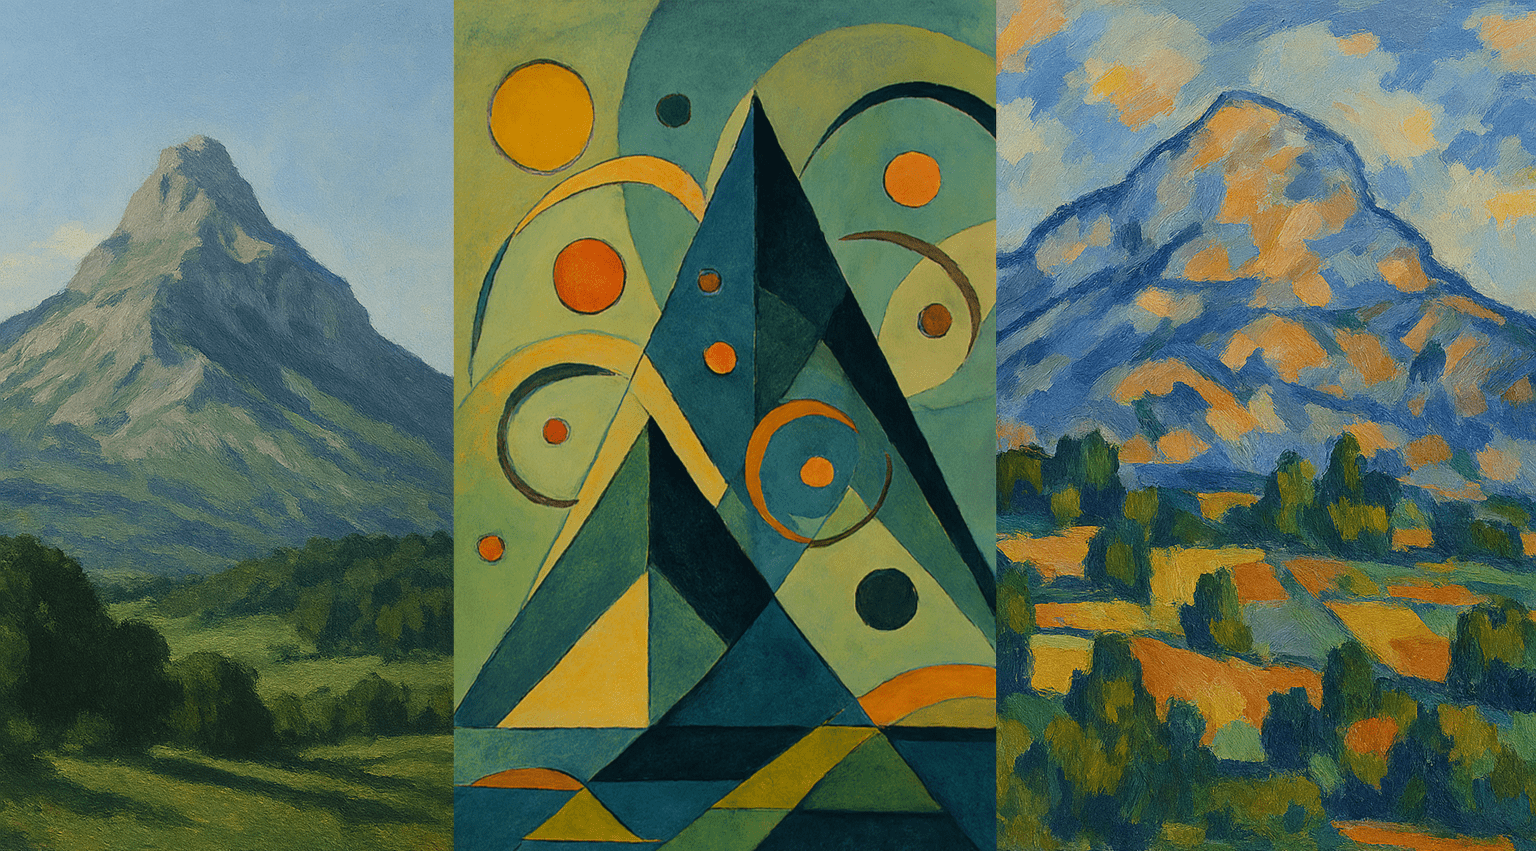
\includegraphics[width=\textwidth]{cover.png}\\[5pt]
 \vfill
{Sep 2025}
\end{center}
\end{titlepage}

{\clearpage

\thispagestyle{empty}
\newlength{\longest}
\settowidth\longest{\huge\itshape Seeing the mountain still as a mountain.}
\null\vfill

\centering
\parbox{\longest}{%
  \raggedright{\huge\itshape%
  Seeing the mountain as the mountain; \\ 
  Seeing the mountain as not a mountain; \\ 
  Seeing the mountain as still a mountain. \par\bigskip
  }   
  \raggedleft\Large\MakeUppercase{Qingyuan Xingsi}\par%
}

\vfill\vfill

\clearpage}

\tableofcontents
\setcounter{chapter}{-1}
\chapter{Introduction}\label{chap:introduction}


\section{What is Algebraic Geometry?}

Algebraic geometry is the study of geometric spaces that locally arise as solutions to polynomial equations. This study can be approached at two levels:

\begin{itemize}
  \item \textbf{Local:} This involves studying the geometric properties of solution sets to polynomial equations. Since we work not only over $\mathbb{R}$ or $\mathbb{C}$ but potentially over arbitrary fields or rings, we must construct a more intrinsic notion of geometry associated with algebra—namely, the spectrum of a ring. This leads to the study of affine varieties and affine schemes, allowing a translation between algebra and geometry.

  \item \textbf{Synthetic:} Analogous to how manifolds generalize open subsets of $\mathbb{R}^n$, we study spaces that are locally isomorphic to affine varieties. This broader perspective leads to the study of varieties and schemes through various formal frameworks.
\end{itemize}

This lecture is part of an algebraic geometry course that emphasizes the second, synthetic level. However, the underlying question—“How can we construct and classify generalized spaces from certain building blocks?”—is relevant across many branches of geometry. Thus, this part can stand alone as a form of \emph{post-modern}\footnote{A commonly accepted definition is “after World War II.”} synthetic geometry.

\section{Essentialism vs. Structuralism}

Synthetic geometry formalizes geometric concepts through axioms that directly address fundamental entities—such as points and lines—rather than relying on a background space like Cartesian coordinates. In contrast to the analytic viewpoint, where every geometric object is composed of points, synthetic geometry treats lines, curves, and other entities as primitive. The focus shifts to the \textbf{relationships} between these objects, such as “a point lies on a line” or “two lines intersect.”

This structuralism perspective emphasizes understanding objects through their interactions. To formalize these relationships, we use \textbf{category theory} and \textbf{sheaf theory}. Moreover, by viewing categories themselves as spaces, we uncover deeper geometric structures. This formalism, developed through algebraic geometry, now plays a central role in various fields: differential geometry, topology, quantum field theory, and beyond.

\section{What is Geometry in Physics?}

Quantum physics connects to both the local and synthetic levels of algebraic geometry:

\begin{itemize}
  \item \textbf{Local:} The concept of the spectrum of a commutative ring originates from $C^*$-algebras and operator theory, both fundamental in quantum physics. The duality between algebra and geometry is already present in the Heisenberg and Schrödinger formulations.

  \item \textbf{Synthetic:} In quantum field theory, we study the space of field configurations (histories), which is infinite-dimensional and behaves irregularly. Nevertheless, we aim to treat it as a “manifold” to define metrics, path integrals, and differential forms. Synthetic geometry provides a rigorous framework for these constructions (e.g., via smooth sets). Gauge theory, supergeometry, and related topics can also be unified within this framework \cite{nlab:geometry_of_physics}.
\end{itemize}

A concrete example is mirror symmetry, which links Gromov–Witten invariants with Hodge theory.

\section{Course Plan}

We will focus on three types of geometry and study them comparatively using synthetic methods:

\begin{itemize}
  \item \textbf{Smooth Sets / Manifolds:} Built from open subsets of $\mathbb{R}^n$, these provide intuitive and geometric examples, serving as a bridge to classical geometry.

  \item \textbf{Simplicial Sets / Kan Complexes:} Constructed from simplices $\Delta$, these offer the simplest and most abstract examples.

  \item \textbf{Algebraic Sets / Schemes:} Built from spectra of commutative rings, these are the central objects of study in this course.
\end{itemize}

\chapter{Category}\label{chap:category} 

There are many references available for category theory; in this course, we follow \cite{nlab:geometry_of_physics_--_categories_and_toposes}
\section{Definition and Examples}
\begin{definition}[Category]
A \textbf{category} $\mathcal{C}$ consists of:
\begin{itemize}
  \item A class of objects $\mathrm{Ob}(\mathcal{C})$.
    \item For each pair $A, B$, a set of morphisms $\mathrm{Hom}_{\mathcal{C}}(A, B)$.
    \item A composition operation $\circ$ of morphisms and identity morphisms $\mathrm{id}_A$ for each object $A$.
\end{itemize}

Subject to:
\begin{itemize}
    \item \textbf{Associativity:} $h \circ (g \circ f) = (h \circ g) \circ f$
    \item \textbf{Identity:} $\mathrm{id}_B \circ f = f = f \circ \mathrm{id}_A$
\end{itemize}
 
\end{definition}

For simplicity, we denote objects in a category $\mathcal{C}$ by $A \in \mathcal{C}$ and morphisms by $f: A \to B$. There are various ways to understand what a category is; let us explore this through examples:

\begin{example}[Concrete Category]
A concrete category can be viewed as a collection of mathematical structures, where morphisms are maps that preserve those structures.
\begin{itemize}
  \item \textbf{Set:} Objects are sets\footnote{Since the collection of all sets does not itself form a set, we refer instead to a \emph{class} of objects. However, if we restrict our attention to \emph{small} sets, then the collection of objects can be treated as a set. In this course, we will ignore set-theoretic subtleties and proceed informally.}; morphisms are functions between sets.
    \item \textbf{Grp:} Objects are groups; morphisms are group homomorphisms.
    \item \textbf{Vect:} Objects are vector spaces; morphisms are linear maps.
    \item \textbf{Top:} Objects are topological spaces; morphisms are continuous maps.
\end{itemize}
You can construct infinitely many examples from the mathematical structures you are familiar with.
\end{example}

At first glance, this abstraction may seem unnecessary. However, we can generalize familiar notions from set theory. For instance, consider a morphism $f: A \to B$ in a category $\mathcal{C}$:

\begin{itemize}
    \item \textbf{Isomorphism:} $f$ is an \emph{isomorphism} if there exists a morphism $g: B \to A$ such that:
    \[
      g \circ f = \mathrm{id}_A \quad \text{and} \quad f \circ g = \mathrm{id}_B (\text{i.e.} g=f^{-1})
    \]
    In this case, $A$ and $B$ are said to be \emph{isomorphic}.

    \item \textbf{Monomorphism:} $f$ is a \emph{monomorphism} (or \emph{mono}) if for all morphisms $g_1, g_2: X \to A$, we have:
    \[
    f \circ g_1 = f \circ g_2 \Rightarrow g_1 = g_2
    \]
    That is, $f$ is left-cancellable.

    \item \textbf{Epimorphism:} $f$ is an \emph{epimorphism} (or \emph{epi}) if for all morphisms $h_1, h_2: B \to Y$, we have:
    \[
    h_1 \circ f = h_2 \circ f \Rightarrow h_1 = h_2
    \]
    That is, $f$ is right-cancellable.

\end{itemize}
\begin{exercise}
Verify that in the category $\Set$, these definitions correspond to bijections, injections, and surjections, respectively.
\end{exercise}

Besides the concrete categories, in which object have its own meaning, we can have abstract categories than objects are meaningless without in the context of category.
\begin{example}[Classifying Category]
  A category can be viewed as an algebraic structure generalizing a monoid\footnote{An algebraic structure similar to a group, but without requiring inverses}. Indeed, for any object $A \in \mathcal{C}$, the set of endomorphisms $\mathrm{Hom}_{\mathcal{C}}(A, A)$ forms a monoid. Conversely, any monoid $M$ can be associated with a \textbf{classifying category} $BM$, which has a single object $\bullet$ and morphisms $\mathrm{Hom}_{BM}(\bullet, \bullet) = M$. In particular, for any group $G$, we obtain a \textbf{classifying space} $BG$, where all morphisms are isomorphisms.
\end{example}

We refer to $BG$ as a space because we can interpret its isomorphisms as paths in a certain topological space:

\begin{example}[Groupoid]
A \textbf{groupoid} is a category in which every morphism is an isomorphism. Given a groupoid $\mathcal{X}$, we can construct its \textbf{geometric realization} $|\mathcal{X}|$ as follows:
\begin{itemize}
    \item Take the objects $x \in \mathcal{X}$ as points.
    \item For each morphism $f: x \to y$, attach a segment from point $x$ to point $y$.
    \item For each relation $f \circ g = h$, attach a triangle with edges labeled by $f$, $g$, and $h$.
    \item Continue this process for higher-dimensional cells $\ldots$
\end{itemize}
We will formalize this construction when we introduce simplicial sets.

\begin{exercise}
Show that the set of connected components $\pi_0(|\mathcal{X}|, x)$ corresponds bijectively to the isomorphism class of $x$ in $\mathcal{X}$. Furthermore, observe that $\mathrm{Hom}_{\mathcal{X}}(x, x)$ is a group, and prove that the fundamental group $\pi_1(|\mathcal{X}|, x) \cong \mathrm{Hom}_{\mathcal{X}}(x, x)$.
\end{exercise}

Conversely, for a topological space $S$, we can define the \textbf{fundamental groupoid} $\Pi_1(S)$, where:
\begin{itemize}
    \item Objects are points of $S$.
    \item Morphisms $\mathrm{Hom}_{\Pi_1(S)}(a, b)$ are homotopy classes of paths from $a$ to $b$.
\end{itemize}

\begin{exercise}
Describe the composition law in $\Pi_1(S)$ and verify that it satisfies the axioms of a groupoid.
\end{exercise}
\end{example}

The examples above illustrate that morphisms in a category can carry rich structure. On the other hand, if morphisms are trivial (i.e., at most one between any two objects), we obtain a partially ordered set:

\begin{example}[Poset]
Let $(P, \leq)$ be a partially ordered set. We can regard $P$ as a category as follows:
\begin{itemize}
    \item \textbf{Objects:} Elements of $P$.
    \item \textbf{Morphisms:} For $x, y \in P$, there exists a unique morphism $f: x \to y$ if and only if $x \leq y$.
    \item \textbf{Composition:} If $x \leq y$ and $y \leq z$, then $x \leq z$, so the morphism $x \to z$ is the composition of $x \to y$ and $y \to z$.
    \item \textbf{Identity:} For each $x \in P$, the identity morphism $\mathrm{id}_x: x \to x$ corresponds to the reflexivity $x \leq x$.
\end{itemize}

This category is called \emph{thin}, meaning there is at most one morphism between any two objects.

A frequently used example is the poset of open subsets of a topological space $S$, denoted $(\mathrm{Op}(S), \subseteq)$.
\end{example}

Note that a set $A$ can be viewed as a category in two distinct ways: either as a trivial groupoid or as a trivial poset. And a category can be viewed as a combination of this two case\footnote{It is useful to think category as an oriented graph}.
% https://q.uiver.app/#q=WzAsNCxbMSwyLCJTZXQiXSxbMCwxLCJHcm91cG9pZCJdLFsyLDEsIlBvc2V0Il0sWzEsMCwiQ2F0ZW9ncnkiXSxbMCwxLCIiLDAseyJzdHlsZSI6eyJ0YWlsIjp7Im5hbWUiOiJob29rIiwic2lkZSI6ImJvdHRvbSJ9fX1dLFswLDIsIiIsMix7InN0eWxlIjp7InRhaWwiOnsibmFtZSI6Imhvb2siLCJzaWRlIjoidG9wIn19fV0sWzEsMywiIiwwLHsic3R5bGUiOnsidGFpbCI6eyJuYW1lIjoiaG9vayIsInNpZGUiOiJ0b3AifX19XSxbMiwzLCIiLDIseyJzdHlsZSI6eyJ0YWlsIjp7Im5hbWUiOiJob29rIiwic2lkZSI6ImJvdHRvbSJ9fX1dXQ==
\[\begin{tikzcd}[ampersand replacement=\&,cramped]
\& \textbf{Category} \\
	\textbf{Groupoid} \&\& \textbf{Poset} \\
	\& \textbf{Set}
	\arrow[hook, from=2-1, to=1-2]
	\arrow[hook', from=2-3, to=1-2]
	\arrow[hook', from=3-2, to=2-1]
	\arrow[hook, from=3-2, to=2-3]
\end{tikzcd}\]

\begin{remark}
In the definition of a category, if we allow the morphism set $\mathrm{Hom}_{\mathcal{C}}(A, B)$ to carry additional structure—such as an Abelian group, vector space, groupoid, topological space, or even another category—we obtain an \textbf{enriched category}. In fact, it is often more natural to think of $\mathrm{Hom}_{\mathcal{C}}(A, B)$ as the set of connected components of a space:
\[
\mathrm{Hom}_{\mathcal{C}}(A, B) \cong \pi_0 \mathrm{Map}_{\mathcal{C}}(A, B).
\]

This reflects a general principle of the \textbf{Univalence Foundation}: mathematical structures should be treated as spaces (or types) from the outset, and the classical set-theoretic version can be recovered by taking the set of connected components. We will explore how to identify and work with these underlying geometric structures later in the course.
\end{remark} 

\section{Functor}

To define a map between two categories, it is natural to require that such a map respects the structure of morphisms.

\begin{definition}[Functor]
Let $\mathcal{C}$ and $\mathcal{D}$ be categories. A \textbf{functor} $F: \mathcal{C} \to \mathcal{D}$ consists of:
\begin{itemize}
    \item A function that assigns to each object $A \in \mathcal{C}$ an object $F(A) \in \mathcal{D}$.
    \item A function that assigns to each morphism $f: A \to B$ in $\mathcal{C}$ a morphism $F(f): F(A) \to F(B)$ in $\mathcal{D}$.
\end{itemize}
such that:
\begin{itemize}
    \item \textbf{Identity preservation:} $F(\mathrm{id}_A) = \mathrm{id}_{F(A)}$.
    \item \textbf{Composition preservation:} For all $f: A \to B$ and $g: B \to C$ in $\mathcal{C}$,
    \[
    F(g \circ f) = F(g) \circ F(f).
    \]
\end{itemize}
\end{definition}

We denote the set (later, the category) of functors from $\mathcal{C}$ to $\mathcal{D}$ by $\mathrm{Fun}(\mathcal{C}, \mathcal{D})$.

\begin{example}[Functors Between Concrete Categories]
Functors between concrete categories respect the underlying structures:
\begin{itemize}
    \item \textbf{Forgetful Functor:}
    \[
    U: \mathbf{Grp} \to \mathbf{Set}
    \]
    assigns to each group its underlying set, and to each group homomorphism the same function viewed as a map of sets. Similar forgetful functors exist for $\mathbf{Vect}$, $\mathbf{Top}$, etc.

    \item \textbf{Free Functor:}
    \[
    \mathrm{Free}: \mathbf{Set} \to \mathbf{Grp}
    \]
    assigns to each set the free group it generates, and to each function between sets the induced group homomorphism.

    \begin{exercise}
    Verify that $\mathrm{Free}$ is indeed a functor. Then show:
    \[
    \mathrm{Hom}_{\mathbf{Grp}}(\mathrm{Free}(A), G) \cong \mathrm{Hom}_{\mathbf{Set}}(A, U(G)).
    \]
    How would you define $\mathrm{Free}$ for $\mathbf{Vect}$?
    \end{exercise}

    \item \textbf{Discrete Functor:}
    \[
    \mathrm{Disc}: \mathbf{Set} \to \mathbf{Top}
    \]
    assigns to each set the discrete topological space, and to each function the same map viewed as continuous.

    \item \textbf{Connected Components:}
    \[
    \pi_0: \mathbf{Top} \to \mathbf{Set}
    \]
    assigns to each topological space its set of connected components.

    \begin{exercise}
    Show:
    \[
    \mathrm{Hom}_{\mathbf{Top}}(\mathrm{Disc}(A), S) \cong \mathrm{Hom}_{\mathbf{Set}}(A, U(S)), \quad
    \mathrm{Hom}_{\mathbf{Top}}(S, \mathrm{Disc}(A)) \cong \mathrm{Hom}_{\mathbf{Set}}(\pi_0(S), A).
    \]
    \end{exercise}
\end{itemize}
\end{example}

\begin{exercise}
  \begin{enumerate}
    \item Let $G, H$ be groups (or more generally, monoids). Show that functors $F: BG \to BH$ correspond bijectively to group (monoid) homomorphisms $f: G \to H$.
    \item Show that a functor $F: BG\to \mathbf{Vect}$ correspond bijectively to representation of $G$.
  \end{enumerate}
\end{exercise}

\begin{exercise}
\begin{enumerate}
    \item Let $\mathcal{X}, \mathcal{Y}$ be groupoids. Show that a functor $F: \mathcal{X} \to \mathcal{Y}$ induces a continuous map between their geometric realizations:
    \[
    |F|: |\mathcal{X}| \to |\mathcal{Y}|.
    \]
    Let $\mathbf{Grpd}$ be the category of groupoids with functors as morphisms. Show that geometric realization defines a functor:
    \[
    |\cdot|: \mathbf{Grpd} \to \mathbf{Top}.
    \]
    \item Similarly, show that the fundamental groupoid construction defines a functor:
    \[
    \Pi_1: \mathbf{Top} \to \mathbf{Grpd}.
    \]
    \item* Show the adjunction:
    \[
    \mathrm{Hom}_{\mathbf{Top}}(S, |\mathcal{X}|) \cong \mathrm{Hom}_{\mathbf{Grpd}}(\Pi_1(S), \mathcal{X}).
    \]
\end{enumerate}
\end{exercise}

\begin{exercise}
Let $P, Q$ be posets. Show that a functor $F: P \to Q$ is equivalent to an order-preserving function.
\end{exercise}

\begin{example}[Ring–Space Correspondence]
Given a topological space $X$, its ring of real continuous functions $C(X)$ defines a contravariant functor. A map $p: X \to Y$ induces a pullback:
\[
p^*: C(Y) \to C(X), \quad f \mapsto f \circ p.
\]
To formalize this, we introduce the \textbf{opposite category} $\mathcal{C}^{\mathrm{op}}$, which has the same objects as $\mathcal{C}$ but reverses the direction of morphisms:
\[
\mathrm{Hom}_{\mathcal{C}^{\mathrm{op}}}(A, B) = \mathrm{Hom}_{\mathcal{C}}(B, A).
\]
Then,
\[
C(-): \mathbf{Top}^{\mathrm{op}} \to \mathbf{Ring}
\]
is a functor.
\end{example}

\begin{remark}
A central theme in algebraic geometry is reversing this functor: constructing a space from a commutative ring. That is, defining a functor:
\[
\mathrm{Spec}: \mathbf{Ring}^{\mathrm{op}} \to \mathbf{Top},
\]
such that we have \emph{adjunction}:
\[
\mathrm{Hom}_{\mathbf{Ring}}(R, C(X)) \cong \mathrm{Hom}_{\mathbf{Top}}(X, \mathrm{Spec}(R)).
\]

\begin{exercise}*
Show that the underlying set of $\mathrm{Spec}(R)$ is:
\[
U(\mathrm{Spec}(R)) = \mathrm{Hom}_{\mathbf{Ring}}(R, \mathbb{R} ).
\]
What topology should be given to $\mathrm{Spec}(R)$?
\end{exercise}

In practice, we impose additional structure to make this correspondence well-behaved:
\begin{itemize}
    \item Between $C^*$-algebras and locally compact Hausdorff spaces, via the Gelfand representation theorem—where the term “spectrum” originates.
    \item Between commutative rings and locally ringed spaces, which is foundational in algebraic geometry.
\end{itemize}
\end{remark}

\begin{example}[Hom Functor]
For a fixed object $A$ in a category $\mathcal{C}$, the \textbf{Hom functor} is defined as:
\[
h^A := \mathrm{Hom}_{\mathcal{C}}(A, -): \mathcal{C} \to \mathbf{Set},
\]
which assigns to each object $B$ the set $\mathrm{Hom}_{\mathcal{C}}(A, B)$, and to each morphism $f: B \to C$ the function:
\[
h^A(f): \mathrm{Hom}_{\mathcal{C}}(A, B) \to \mathrm{Hom}_{\mathcal{C}}(A, C), \quad g \mapsto f \circ g.
\]
Similarly, we define the contravariant version:
\[
h_A := \mathrm{Hom}_{\mathcal{C}}(-, A): \mathcal{C}^{\mathrm{op}} \to \mathbf{Set}.
\]
\end{example}

\begin{exercise}
Show that:
\begin{itemize}
    \item $f$ is a monomorphism if and only if $h^A(f)$ is injective for all $A$.
    \item $f$ is an epimorphism if and only if $h_A(f)$ is injective for all $A$.
    \item $f$ is an isomorphism if and only if both $h^A(f)$ and $h_A(f)$ are bijective for all $A$.
\end{itemize}
\end{exercise}

\begin{remark}
We can think of objects in $\mathcal{C}$ as “test objects,” and a functor as a way of encoding data about how these tests behave. For example, in a sigma model with target space $M$, let $\mathcal{C}$ be the category of space-times. For each space-time $\Sigma$, the collection of fields $\mathrm{Map}(\Sigma, M)$ defines such a functor. The fundamental question is: given such a functor, can we reconstruct the underlying “space”?
\end{remark}

\section{Presheaf}

We now introduce a central concept for understanding "generalized spaces" in this course.

\begin{definition}[Presheaf]
Let $\mathcal{C}$ be a category. A \textbf{presheaf} on $\mathcal{C}$ is a functor:
\[
F: \mathcal{C}^{\mathrm{op}} \to \mathbf{Set}
\]
That is, $F$ assigns:
\begin{itemize}
    \item To each object $U$ in $\mathcal{C}$, a set $F(U)$.
    \item To each morphism $f: V \to U$ in $\mathcal{C}$, a function:
    \[
    F(f): F(U) \to F(V)
    \]
\end{itemize}
such that:
\begin{itemize}
    \item $F(\mathrm{id}_U) = \mathrm{id}_{F(U)}$
    \item $F(g \circ f) = F(f) \circ F(g)$ for composable morphisms $f$ and $g$ in $\mathcal{C}$
\end{itemize}
\end{definition}

Let $\PSh(\mathcal{C}) = \mathrm{Fun}(\mathcal{C}^{\mathrm{op}}, \mathbf{Set})$ denote the category of presheaves on $\mathcal{C}$.

\begin{remark}
To understand why presheaves represent generalized spaces, consider the analogy with distributions as generalized functions:
\begin{itemize}
    \item We begin with a space of test functions. Let $\mathcal{D}(\Omega)$ denote the space of smooth functions with compact support in $\Omega$. There is a natural pairing:
    \[
    \langle f, g \rangle := \int_\Omega f g
    \]
    This allows us to associate to each test function $f \in \mathcal{D}(\Omega)$ a continuous functional $T_f \in \mathcal{D}'(\Omega)$ defined by:
    \[
    T_f(\phi) := \int_\Omega f \phi.
    \]
    The space $\mathcal{D}'(\Omega)$ of distributions is thus a space of generalized functions.

    \item Similarly, starting from a category of test spaces $\mathcal{C}$, we consider the Hom functor:
    \[
    \mathrm{Hom}_{\mathcal{C}}(-, -): \mathcal{C}^{\mathrm{op}} \times \mathcal{C} \to \mathbf{Set}.
    \]
    For each object $A \in \mathcal{C}$, the presheaf $h_A := \mathrm{Hom}_{\mathcal{C}}(-, A)$ is \emph{representable}. Presheaves generalize these representable ones, just as distributions generalize smooth functions.

    \item In solving differential equations, we often first obtain a distributional solution, and then study its \emph{regularity}—how closely it resembles a smooth function locally—allowing us to conclude that the distribution is an actual function.

    \item In geometry, for example in moduli problems, we may first define a (pre)sheaf\footnote{sheaf to presheaf, is like continuous functional to functional, we ask some continuous condition on presheaf} and then study its \emph{representability}—whether it locally resembles a test space—allowing us to conclude that we have constructed an actual space.
\end{itemize}
\end{remark}

As we've seen, for any $A \in \mathcal{C}$, the presheaf $h_A$ is called representable. Just as there are distributions that are not smooth functions, there are presheaves that are not representable. Here are some concrete examples:

\begin{example}[Presheaf of Functions]
Let $X$ be a topological space. For each open set $U \in \mathrm{Op}(X)$, the set of continuous functions $C(U)$ defines a presheaf $C \in \PSh(\mathrm{Op}(X))$. For $U \subseteq V$, we have a restriction map $C(V) \to C(U)$. More generally, for any topological space $Y$, we can define a presheaf $C(-, Y) \in \PSh(\mathrm{Op}(X))$. Similarly, one can define presheaves of smooth, analytic, or locally constant functions.
\end{example}

\begin{example}[Presheaf of Sections]
Let $E \to X$ be a vector bundle over a topological space $X$. Define the presheaf of sections $\Gamma_E$ by assigning to each open set $U \subseteq X$ the set of continuous (or smooth) sections of $E$ over $U$:
\[
\Gamma_E(U) = \{ s : U \to E \mid s \text{ is a section of } E \text{ over } U \}.
\]
\end{example}

\begin{example}[Smooth Set]
Let $\Cart$ be the category of Cartesian spaces, with objects $\mathbb{R}^n$ and morphisms given by smooth maps. A presheaf on $\Cart$ is called a \textbf{smooth set}.
\begin{itemize}
  \item \textbf{Manifolds:} For any smooth manifold $M$, define a presheaf $M(\mathbb{R}^n) := \{f: \mathbb{R}^n\to M \mid f \text{ is smooth.}\}$. Thus, every manifold defines a smooth set.
  \item \textbf{Differential Forms:} Consider the presheaf $\Omega^k$ assigning to each $\mathbb{R}^n$ the space of $k$-forms $\Omega^k(\mathbb{R}^n)$, with pullbacks along smooth maps. Show that $\Omega^k$ is not representable by a manifold.
\end{itemize}
\end{example}

\begin{example}[Simplicial Set]
  example
\end{example}

\begin{example}[Algebraic Set]
In algebraic geometry, we treat $\mathbf{Ring}^{\mathrm{op}}$ as the category of test spaces. A presheaf $\mathcal{F} \in \PSh(\mathbf{Ring}^{\mathrm{op}}) = \mathrm{Fun}(\mathbf{Ring}, \mathbf{Set})$ is then a functor from rings to sets, which we call an \textbf{algebraic set}.
\begin{itemize}
    \item \textbf{Affine Variety:} We begin with the geometry of zero set of polynomials. Let $P_1, \ldots, P_m \in \mathbb{Z}[x_1, \ldots, x_n]$ be polynomials. Define a functor $V_P: \mathbf{Ring} \to \mathbf{Set}$ by:
    \[
    V_P(R) = \{ (r_1, \ldots, r_n) \in R^n \mid P_i(r_1, \ldots, r_n) = 0 \text{ for all } i \}.
    \]
    \begin{exercise}
    Let $R_P = \mathbb{Z}[x_1, \ldots, x_n]/(P_1, \ldots, P_m)$. Show that $V_P = h^{R_P}$, i.e., $V_P(R) = \mathrm{Hom}_{\mathbf{Ring}}(R_P, R)$.
    \end{exercise}

    \item \textbf{Projective Space:} Then we consider a non-representable example. Define a functor $\mathbb{P}^n: \mathbf{Ring} \to \mathbf{Set}$ by:
    \[
    \mathbb{P}^n(R) = \{ (r_0, \ldots, r_n) \in R^{n+1} \mid \exists (u_0, \ldots, u_n) \in R^{n+1} \text{ s.t. } \sum u_i r_i = 1 \}/\sim,
    \]
    where $\sim$ identifies tuples under scalar multiplication by units in $R$.

    \begin{exercise}
    Show that this defines a functor. Compare this with the definition of projective space in differential geometry when $R = \mathbb{R}$.
    \end{exercise}
\end{itemize}
\end{example}

As we indicated earlier, $\PSh(\mathcal{C})$ should itself form a category. Let us now determine what the morphisms between presheaves ought to be.

Since representable presheaves $h_A$ and $h_B$ are thought of as generalized spaces, it is natural to expect that morphisms between them should reflect the morphisms in the original category $\mathcal{C}$. Indeed, given a morphism $f: A \to B$ in $\mathcal{C}$, we can define a map of sets:
\[
f \circ - : h_A(C) \to h_B(C), \quad \text{for each } C \in \mathcal{C},
\]
However, for this to define a morphism of presheaves, these maps must be compatible with the structure of the presheaves—i.e., they must commute with the restriction maps for all choices of $C$ and morphisms between them.

This leads us naturally to the definition of morphisms between presheaves as \emph{natural transformations}, which ensure such compatibility across the entire category.

\begin{definition}[Morphisms of Presheaves]
A \emph{morphism of presheaves} $\varphi: \mathcal{F} \to \mathcal{G}$ is a natural transformation between the functors $\mathcal{F}$ and $\mathcal{G}$. That is, for each object $U$ in $\mathcal{C}$, there is a function $\varphi_U: \mathcal{F}(U) \to \mathcal{G}(U)$ such that for every morphism $f: V \to U$ in $\mathcal{C}$, the following diagram commutes:
% https://q.uiver.app/#q=WzAsNCxbMCwwLCJcXGJ1bGxldCJdLFsxLDAsIlxcYnVsbGV0Il0sWzAsMSwiXFxidWxsZXQiXSxbMSwxLCJcXGJ1bGxldCJdLFswLDEsIlxcdmFycGhpX1UiXSxbMCwyLCJcXG1hdGhjYWx7Rn0oZikiLDJdLFsyLDMsIlxcdmFycGhpX1YiXSxbMSwzLCJcXG1hdGhjYWx7R30oZikiXV0=
\[\begin{tikzcd}[ampersand replacement=\&,cramped]
  \mathcal{F}(U) \&  \mathcal{G}(U) \\
\mathcal{F}(V)   \& \mathcal{G}(V)
	\arrow["{\varphi_U}", from=1-1, to=1-2]
	\arrow["{\mathcal{F}(f)}"', from=1-1, to=2-1]
	\arrow["{\mathcal{G}(f)}", from=1-2, to=2-2]
	\arrow["{\varphi_V}", from=2-1, to=2-2]
\end{tikzcd}\]

\end{definition}
\begin{exercise}
\begin{enumerate}
    \item Show that a morphism $f: A \to B$ in $\mathcal{C}$ induces a morphism of presheaves $\yo(f): h_A \to h_B$. This defines a functor:
    \[
    \yo: \mathcal{C} \to \PSh(\mathcal{C}), \quad A \mapsto h_A,
    \]
    called the \emph{Yoneda embedding}.
    \item* (Yoneda Lemma) Show that, for $A\in \cC$ and $F\in \PSh(\cC)$ there is a bijection:
    \[
     F(A) \cong \mathrm{Hom}_{\PSh(\mathcal{C})}(h_A, F).
    \]
    As a corollary, for any $A,B\in \cC$ there is a bijection of morphisms:
    \[
    \yo(-): \mathrm{Hom}_{\mathcal{C}}(A, B) \cong \mathrm{Hom}_{\PSh(\mathcal{C})}(h_A, h_B).
    \]
\end{enumerate}
\end{exercise}

This lemma is extremely important. It justifies embedding the category $\mathcal{C}$ into the category of presheaves $\PSh(\mathcal{C})$ in a way that fully preserves its morphism structure. In other words, $\mathcal{C}$ can be faithfully represented inside $\PSh(\mathcal{C})$ via the Yoneda embedding.
\begin{exercise}
  \begin{enumerate}
    \item 
Let $M$ be a smooth manifold viewed as a smooth set. Show that every differential form $\omega \in \Omega^k(M)$ induces a morphism of smooth sets:
\[
\omega: M \to \Omega^k.
\]
\item* Then prove that this defines a bijection:
\[
\Omega^k(M) \cong \mathrm{Hom}_{\mathrm{sm}}(M, \Omega^k).
\]
  \end{enumerate}
\end{exercise}

\begin{exercise}[Smooth Algebras]
  
   Let smooth algebras $C^{\infty}\mathbf{Alg}$ to be the product preserving functors $A:\Cart \to \Set$. 
    \begin{enumerate}
      \item Show that $A(\bR)$ has a ring structure.
      \item Show that for any smooth manifold $M$ define a smooth algebra $C^\infty(M): \bR^i \mapsto C^\infty(M, \bR^i)$. Thus, every manifold contravariantly defines a smooth algebra.

      \item We have a functor from smooth sets to smooth algebras 
    \[
      C^\infty: \PSh(\Cart) \to C^{\infty}\mathbf{Alg}^\op, X \mapsto \left( \bR^i \mapsto \Hom_{\PSh(\Cart)}(X,\yo \bR^i) \right)
    \]
    and a functor from smooth algebras to smooth algebras

    \[
      \Spec:   C^{\infty}\mathbf{Alg}^\op \to \PSh(\Cart), A \mapsto \left( \bR^i \mapsto \Hom_{C^{\infty}\mathbf{Alg}}(A, C^\infty(\bR^i) ) \right)
    \]
Then show that we have adjunction:
\[
\mathrm{Hom}_{C^{\infty}\mathbf{Alg}}(A, C^\infty(X)) \cong \mathrm{Hom}_{\PSh(\Cart)}(X, \mathrm{Spec}(A)).
\]
    \end{enumerate}
\end{exercise}


\bibliographystyle{plain}
\bibliography{references}
\end{document}
